% Adjust these for the path of the theme and its graphics, relative to this file
%\usepackage{beamerthemeFalmouthGamesAcademy}
\usepackage{../../beamerthemeFalmouthGamesAcademy}
\usepackage{multimedia}
\graphicspath{ {../../} }

% Default language for code listings
\lstset{language=C++,
        morekeywords={each,in,nullptr}
}

% For strikethrough effect
\usepackage[normalem]{ulem}
\usepackage{wasysym}

\usepackage{pdfpages}

\usepackage[skip=2pt,font=tiny]{caption}

% http://www.texample.net/tikz/examples/state-machine/
\usetikzlibrary{arrows,automata}

\hypersetup{
	colorlinks=true,
	linkcolor=gray,
	urlcolor=gray
}

\newcommand{\modulecode}{COMP260}\newcommand{\moduletitle}{Distributed Systems}\newcommand{\sessionnumber}{5}

\begin{document}
\title{\sessionnumber: Introduction to Graphics and Simulation}
\subtitle{\modulecode: \moduletitle}

\frame{\titlepage} 

\begin{frame}
	\frametitle{Learning outcomes}
	By the end of this week, you will be able to:
	\begin{itemize}
		\item \textbf{Understand} the context of computer graphics and simulation in games.
		\item \textbf{Recall} some of the main areas of interest in graphics and simulation.
	\end{itemize}
\end{frame}

\part{Computer graphics}
\frame{\partpage}

\begin{frame}{What is computer graphics?}
	\begin{itemize}
		\pause\item The process of representing 3D virtual objects on a screen.
		\pause\item "The creation of, manipulation of, analysis of, and interaction with pictorial representations of objects and data using computers." \textit{-- Dictionary of Computing}
		\pause\item Trying to make it look as convincing and/or interesting as possible:
		\begin{itemize}
			\pause\item Shape representation - \textbf{modelling}
			\pause\item How light interacts with the surface - \textbf{shading}
			\begin{itemize}
				\pause\item (Photo)realistic vs. stylised, e.g. cel shading
			\end{itemize}
			\pause\item How light travels around the scene - \textbf{rendering}
		\end{itemize}
	\end{itemize}
\end{frame}

\begin{frame}{Modelling}
	\begin{columns}
		\begin{column}{0.3\textwidth}
			\begin{figure}
				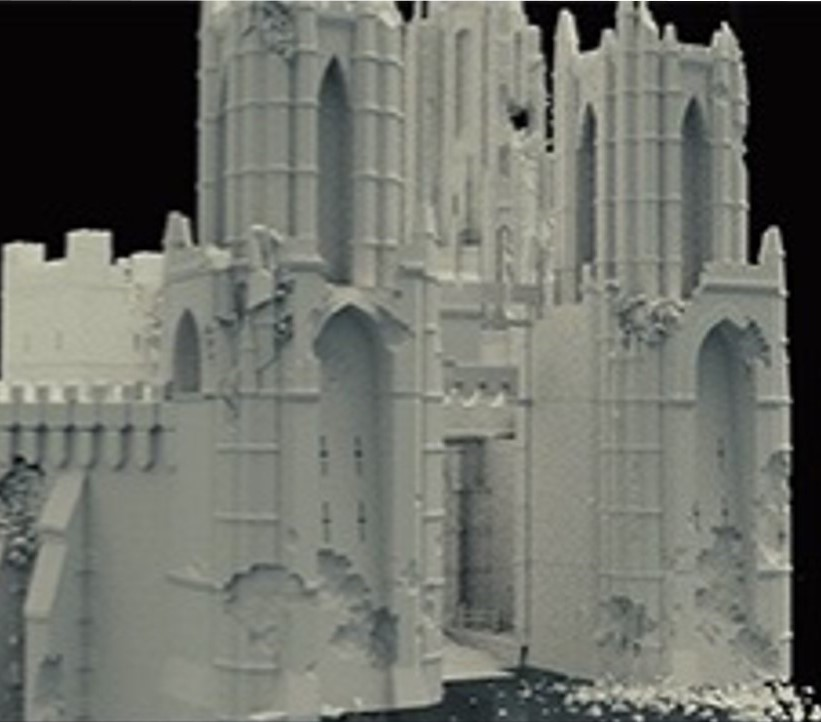
\includegraphics[width=\textwidth]{castle_model}
				\caption*{Image courtesy of \href{https://www.framestore.com}{Framestore}}
			\end{figure}
		\end{column}
		\begin{column}{0.65\textwidth}
			\begin{itemize}
				\pause\item Defines the outline/shape of an object, usually by identifying points or \textbf{vertices} on its surface
				\pause\item Vertices can be generated by an artist using a 3D modelling package, or may be generated procedurally
				\pause\item More vertices => more accurate shape => more data and longer processing times
				\pause\item Algorithms can be used to reduce model complexity without compromising appearance
			\end{itemize}
		\end{column}
	\end{columns}
\end{frame}

\begin{frame}{Shading and rendering}
	\begin{columns}
		\begin{column}{0.3\textwidth}
			\begin{figure}
				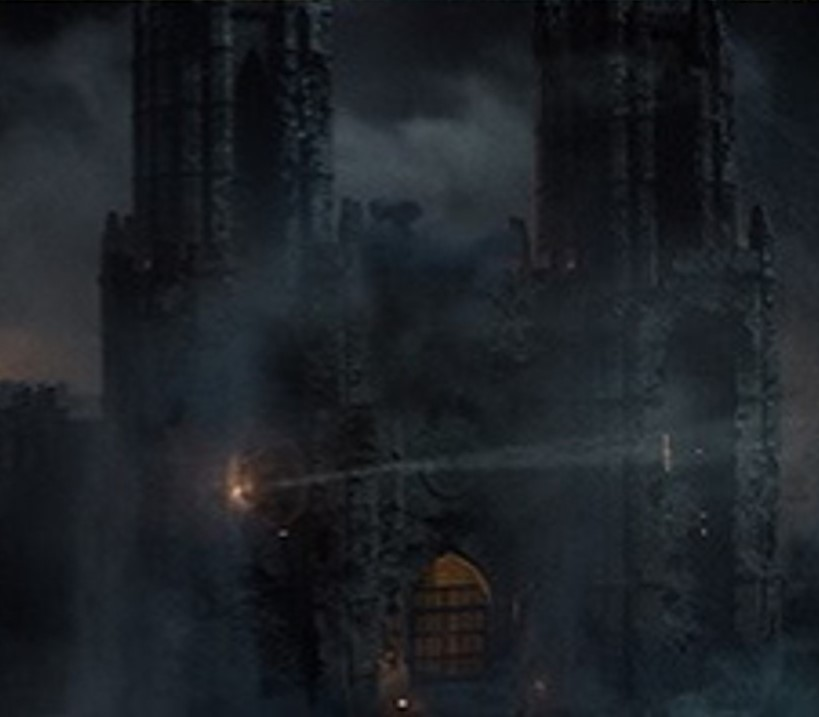
\includegraphics[width=\textwidth]{castle_render}
				\caption*{Image courtesy of \href{https://www.framestore.com}{Framestore}}
			\end{figure}
		\end{column}
		\begin{column}{0.65\textwidth}
			\begin{itemize}
				\pause\item Models are given \textbf{textures} and other surface properties as \textbf{materials}
				\pause\item Use equations from physics to define how light behaves and interacts with materials
				\pause\item A variety of simplifications exist that approximate (some of) the full equation, e.g. Phong shading
			\end{itemize}
		\end{column}
	\end{columns}
\end{frame}

\part{Simulation}
\frame{\partpage}

\begin{frame}{What is simulation?}
	\begin{itemize}
		\pause\item Replicating (physical) behaviour using equations (e.g. Newton's Laws of Motion).
		\pause\item Different kinds of objects behave differently:
		\begin{itemize}
			\pause\item Motion through space resulting from external forces - \textbf{particle simulation}
			\pause\item Changes in orientation resulting from external forces - \textbf{rigid body dynamics}
			\pause\item Changes in shape resulting from external \textit{and internal} forces - \textbf{soft-body deformation}
			\begin{itemize}
				\pause\item Some types of object have specific techniques, e.g. \textbf{hair, cloth} and \textbf{fluid}
			\end{itemize}
			\pause\item Automating aspects of manual animation processes - e.g. \textbf{inverse kinematics (IK)}
		\end{itemize}
	\end{itemize}
\end{frame}

\begin{frame}{Particle simulation}
	\begin{columns}
		\begin{column}{0.3\textwidth}
			\begin{figure}
				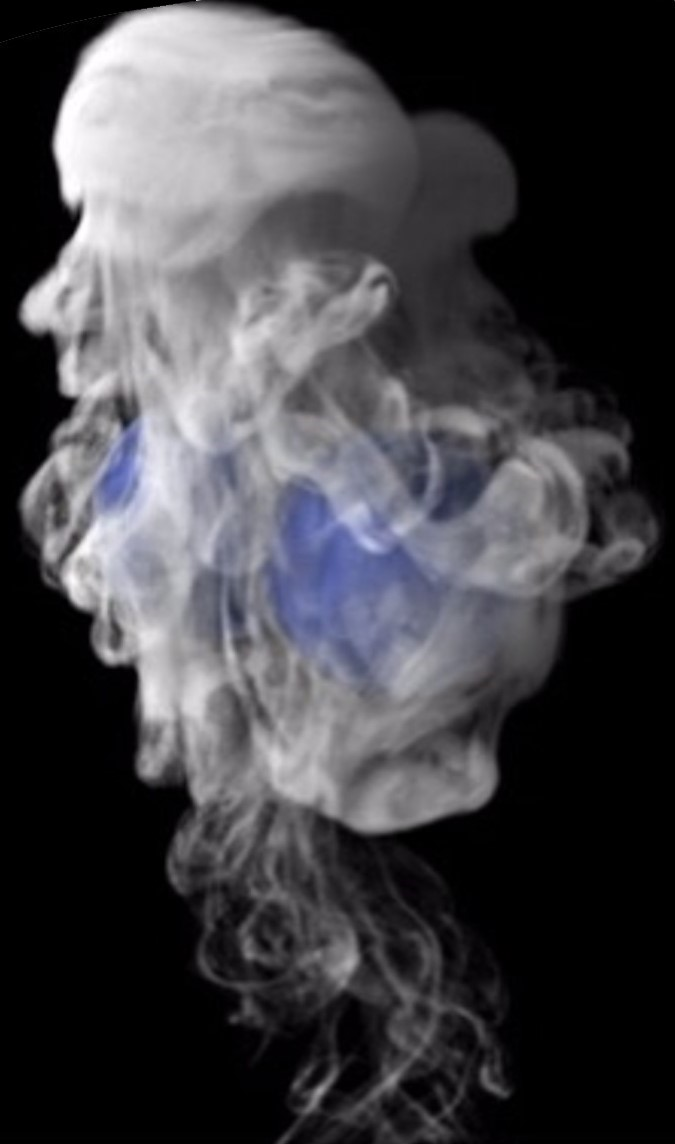
\includegraphics[width=\textwidth]{particles}
				\caption*{Image courtesy of \href{https://www.framestore.com}{Framestore}}
			\end{figure}
		\end{column}
		\begin{column}{0.65\textwidth}
			\begin{itemize}
				\pause\item Used to predict the behaviour of dimensionless \textbf{point mass} objects
				\pause\item Computed one frame at a time, to account for \textbf{collisions}
				\pause\item Can be used for fluid-like effects such as smoke
			\end{itemize}
		\end{column}
	\end{columns}
\end{frame}

\begin{frame}{Rigid body dynamics}
	\begin{columns}
		\begin{column}{0.3\textwidth}
			\begin{figure}
				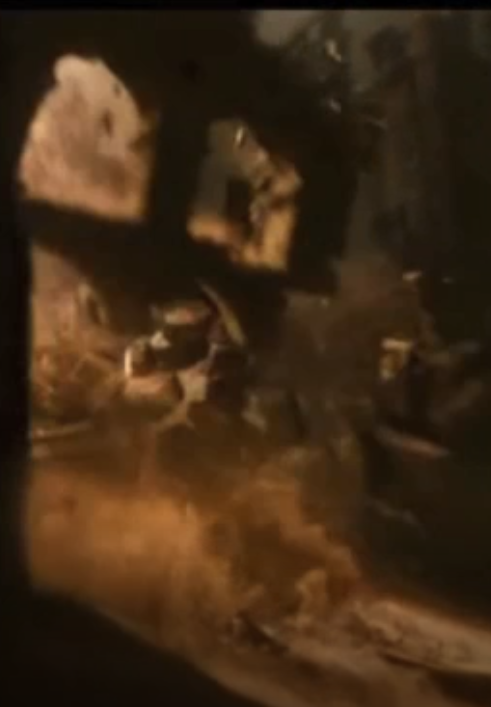
\includegraphics[width=\textwidth]{rigid_bodies}
				\caption*{Image courtesy of \href{https://www.framestore.com}{Framestore}}
			\end{figure}
		\end{column}
		\begin{column}{0.65\textwidth}
			\begin{itemize}
				\pause\item Used to predict the behaviour of \textbf{non-deformable} objects
				\pause\item Global motion is computed as for particles...
				\pause\item ... combined with local motion (rotation) about the object's centre of mass
				\pause\item Commonly used for destruction sequences
			\end{itemize}
		\end{column}
	\end{columns}
\end{frame}

\begin{frame}{Soft body dynamics}
	\begin{columns}
		\begin{column}{0.3\textwidth}
			\begin{figure}
				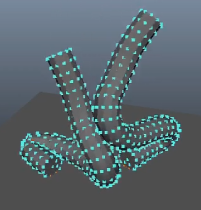
\includegraphics[width=\textwidth]{soft_bodies}
				\caption*{Image courtesy of \href{https://www.framestore.com}{Framestore}}
			\end{figure}
		\end{column}
		\begin{column}{0.65\textwidth}
			\begin{itemize}
				\pause\item Used to predict the behaviour of \textbf{deformable} objects
				\pause\item Requires knowledge of the interior of an object (e.g. FEM): computationally very expensive
				\pause\item Often approximated using \textbf{constrained rigid bodies} and other techniques
			\end{itemize}
		\end{column}
	\end{columns}
\end{frame}

\begin{frame}{Other types of dynamic simulation}
	\begin{columns}
		\begin{column}{0.3\textwidth}
			\begin{figure}
				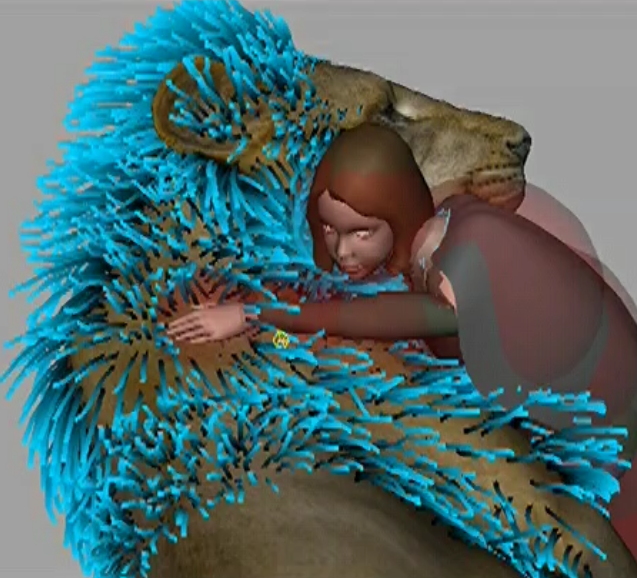
\includegraphics[width=\textwidth]{hair}
				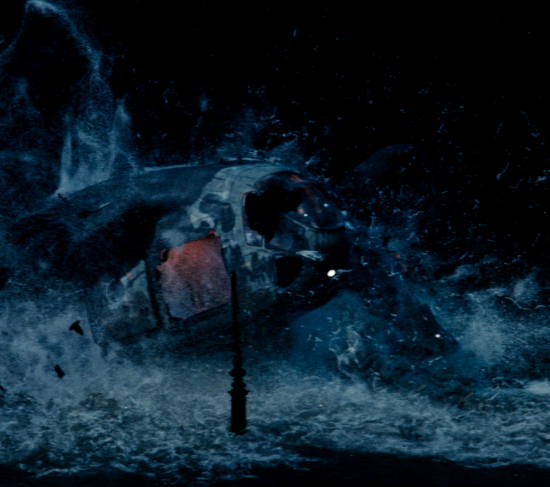
\includegraphics[width=\textwidth]{fluid}
				\caption*{Images courtesy of \href{https://www.framestore.com}{Framestore}}
			\end{figure}
		\end{column}
		\begin{column}{0.65\textwidth}
			\begin{itemize}
				\pause\item Objects such as \textbf{hair, cloth} and \textbf{liquids} behave slightly differently
				\pause\item These have their own equations and techniques...
				\pause\item Beyond the scope of this module!
			\end{itemize}
		\end{column}
	\end{columns}
\end{frame}

\begin{frame}{Rigging and animation}
	\begin{columns}
		\begin{column}{0.3\textwidth}
			\begin{figure}
				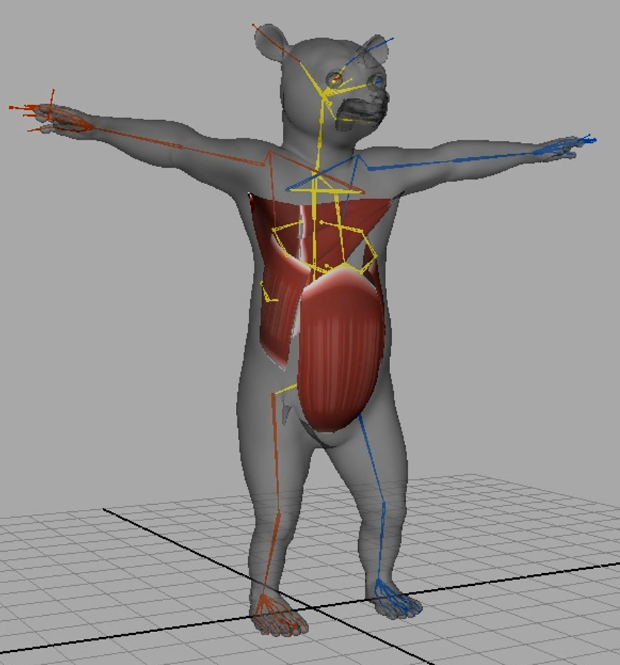
\includegraphics[width=\textwidth]{rigging}
				\caption*{Image courtesy of \href{https://www.framestore.com}{Framestore}}
			\end{figure}
		\end{column}
		\begin{column}{0.65\textwidth}
			\begin{itemize}
				\pause\item Key characters (and objects) are hand-animated by artists using a \textbf{skeleton rig}
				\pause\item Positioning each joint would be a laborious process...
				\pause\item Techniques such as Inverse Kinematics (IK) have been developed to automate certain aspects.
			\end{itemize}
		\end{column}
	\end{columns}
\end{frame}

\part{Context and applications}
\frame{\partpage}

\begin{frame}{Why are graphics and simulation important?}
	\begin{itemize}
		\pause\item More than 50\% of the cortex, the surface of the brain, is devoted to processing visual information (David R. Williams, William G. Allyn Professor of Medical Optics at the University of Rochester; reference \href{William G. Allyn Professor of Medical Optics}{here}).
		\pause\item Most computer output appears on the screen.
		\pause\item Enables intuitive observation of data, representing:
		\begin{itemize}
			\pause\item locations, orientations and dimensions of objects in space
			\pause\item statistical or experimental results
		\end{itemize}
	\end{itemize}
\end{frame}

\begin{frame}{Applications}
	\begin{itemize}
		\pause\item Entertainment: games, virtual reality, films/TV
		\pause\item Architecture and CAD
		\pause\item Engineering
		\pause\item Science and medicine
	\end{itemize}
\end{frame}

\begin{frame}{Challenges}
	\begin{itemize}		
		\pause\item Accuracy vs. speed: complex calculations take time...
		\pause\item Solution: use approximations, considering:
		\begin{itemize}
			\pause\item Which objects do we really need to see?
			\pause\item How much detail do we need to see them in?
			\pause\item What can be sacrificed without compromising the end result (too much)?
		\end{itemize}
		\pause\item Optimisations are possible at each stage of the graphics pipeline
		\pause\item Different applications require different balances of trade-offs; in games, speed is paramount (but detail is desirable!)
	\end{itemize}
\end{frame}


\begin{frame}
	\frametitle{Next steps}
	Now you have a general idea of what graphics and simulation is about, and the factors to bear in mind whilst implementing the techniques,
	\begin{itemize}
		\item \textbf{Review} content from COMP270 on the graphics pipeline.
		\item \textbf{Research} the main topics within graphics and simulation to decide which areas you'd like to focus on for your artefact.
	\end{itemize}
\end{frame}

\end{document}
